\section{Animation}

TODO: einleitung etc.

Ein Layer wird grundsätzlich in zwei Bereiche aufgeteilt. Es gibt den Inputbereich, welcher den
Status eines variablen Objektes vor der Energieübertragung, sowie den Outputbereich, welcher den Status
eines variablen Objektes nach der Energieübertragung beschreibt.

Ein Layer definiert immer deren zwei Keyframes, sofern es sich nicht um den Input- oder Output-Layer handelt.
Um den Zustand des Systems zu einem beliebigen Zeitpunkt zu berechnen, kann
jeweils zwischen den KeyFrames $n$ und $n + 1$ zweier Layer interpoliert werden.

\begin{figure}[h!]
    \begin{center}
        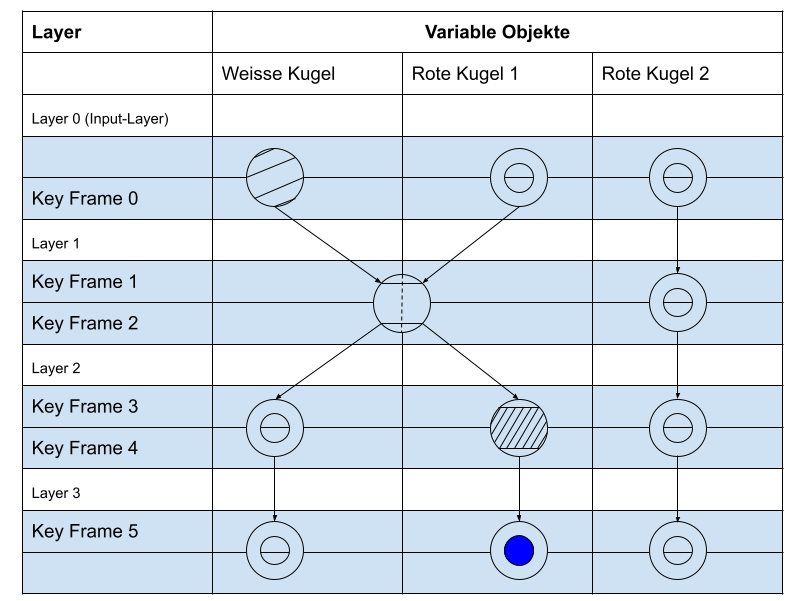
\includegraphics[width=0.5\linewidth]{../common/03_billiard_ai/resources/18_animation_keyframes.png}
    \end{center}
    \caption{Animation keyframes}
    \label{fig:animation_keyframes_example}
\end{figure}
